
\chapter{Radiación Solar\label{cha:Radiacion}}


\section{Naturaleza de la radiación solar}


\subsection{Radiación fuera de la atmósfera terrestre}

La radiación emitida por el Sol atraviesa el espacio vacío en todas
direcciones. No sufre pérdidas apreciables por interacción con medios
materiales. Sin embargo, la irradiancia solar, definida como la densidad
de flujo radiante solar%
\footnote{La irradiancia solar es la \emph{potencia} de radiación solar por
unidad de área incidente en una superficie. Sus unidades en el S.I.
son $\si{\watt\per\meter\squared}$. La irradiación solar es la integral
durante un período temporal de la irradiancia y, por tanto, es la
\emph{energía} de radiación solar por unidad de área incidente en
una superficie. Sus unidades en el S.I. son $\si{\Wh\per\meter\squared}$.%
}, es atenuada de acuerdo con el cuadrado de la distancia. Parte de
esta irradiancia solar es interceptada por el planeta Tierra. Dada
la relación entre la distancia con el Sol y el tamaño de nuestro planeta,
es razonable asumir que su valor es constante en toda la superficie
exterior de nuestra atmósfera. Se define la constante solar, $B_{0}$
\nomenclature[B0]{$B_{0}$}{Constante solar o irradiancia solar incidente en un plano normal al vector solar en el límite superior de la atmósfera terrestre},
como el valor de irradiancia solar incidente en un plano normal al
vector Sol-Tierra en el límite superior de la atmósfera terrestre.
Diferentes campañas de medidas han obtenido valores diferentes para
la constante solar, pero se acepta como representativo el valor promedio
de $B_{0}=\SI{1367}{\watt\per\meter\squared}$ propuesto por la Organización
Meteorológica Mundial.

Como hemos expuesto en el capítulo dedicado a la geometría solar,
la distancia entre la Tierra y el Sol varía a lo largo del año debido
a la excentricidad de la elipse. Esta variación influye en la irradiancia
solar que alcanza la atmósfera. Teniendo en cuenta este hecho, para
calcular la irradiancia incidente en una superficie tangente a la
atmósfera en una latitud determinada emplearemos la ecuación \ref{eq:Bo0}:

\begin{equation}
B_{0}(0)=B_{0}\cdot\epsilon_{0}\cdot\cos\theta_{zs}\label{eq:Bo0}\end{equation}
\nomenclature[Bo0]{$B_{0}(0)$}{Irradiancia extra-atmosférica o extra-terrestre en el plano horizontal}

Este valor, denominado como irradiancia extra-atmosférica o extra-terrestre
en el plano horizontal, representa el valor límite alcanzable en la
superficie terrestre en un plano horizontal. Es importante resaltar
que el valor de la irradiancia extra-atmosférica sólo requiere consideraciones
geométricas. Así, podemos calcular la irradiación diaria extra-atmosférica
integrando la ecuación \ref{eq:Bo0}, y obteniendo la ecuación \ref{eq:Bo0d}:

\begin{equation}
B_{0d}(0)=-\frac{T}{\pi}B_{0}\epsilon_{0}\cdot\left(\omega_{s}\sin\phi\sin\delta+\cos\delta\cos\phi\sin\omega_{s}\right)\label{eq:Bo0d}\end{equation}
\nomenclature[Bod0]{$B_{0d}(0)$}{Irradiación diaria extra-atmosférica o extra-terrestre en el plano horizontal}donde
$\omega_{s}$ está en radianes y $T$ es la duración del día en horas. 

Es posible demostrar que el promedio mensual de esta irradiación
diaria coincide numéricamente con el valor de irradiación diaria
correspondiente a los denominados ``días promedios'', días en los que
la declinación correspondiente coincide con el promedio mensual (tabla
\ref{tab:DiasPromedio}).  Por tanto, podemos calcular el valor medio
mensual de la irradiación diaria extra-atmosférica sin más que incluir
en la ecuación \ref{eq:Bo0d} el valor de la declinación de uno de los
doce días promedio.

\begin{center}
{\footnotesize }%
\begin{table}
{\footnotesize \caption{Valor $d_{n}$ correspondiente a los doce días promedio.\label{tab:DiasPromedio}}
}{\footnotesize \par}

\centering{}{\footnotesize }\begin{tabular}{>{\centering}p{6mm}>{\centering}m{4mm}>{\centering}m{4mm}>{\centering}m{4mm}>{\centering}m{4mm}>{\centering}m{4mm}>{\centering}m{4mm}>{\centering}m{4mm}>{\centering}m{4mm}>{\centering}m{4mm}>{\centering}m{4mm}>{\centering}m{4mm}>{\centering}m{3mm}}
\toprule 
{\footnotesize Mes} & {\footnotesize Ene} & {\footnotesize Feb} & {\footnotesize Mar} & {\footnotesize Abr} & {\footnotesize May} & {\footnotesize Jun} & {\footnotesize Jul} & {\footnotesize Ago} & {\footnotesize Sep} & {\footnotesize Oct} & {\footnotesize Nov} & {\footnotesize Dic}\tabularnewline
\midrule
$d_{n}$ & {\footnotesize 17} & {\footnotesize 45} & {\footnotesize 74} & {\footnotesize 105} & {\footnotesize 135} & {\footnotesize 161} & {\footnotesize 199} & {\footnotesize 230} & {\footnotesize 261} & {\footnotesize 292} & {\footnotesize 322} & {\footnotesize 347}\tabularnewline
\bottomrule
\end{tabular}
\end{table}

\par\end{center}{\footnotesize \par}


\subsection{Influencia de la atmósfera terrestre en la radiación solar}

A su paso por la atmósfera, la radiación solar es sometida a una
combinación de procesos de reflexión, atenuación y difusión que
alteran sus características.  La reflexión en las nubes disminuye la
radiación incidente en la superficie terrestre mientras que la
absorción por vapor de agua, ozono y $\mathrm{CO}_2$ produce una
modificación de las características espectrales de la
radiación. Además, la dispersión por partículas modifica la
distribución espacial de la radiación. Dependiendo del tamaño de la
partícula en interacción pueden distinguirse tres fenómenos de
difusión:
\begin{itemize}
\item Difusión de Rayleigh, donde la longitud de onda es mucho mayor
  que el tamaño de la partícula. Se produce en las capas altas y es responsable
del color azul del cielo.
\item Difusión de Mie, donde la longitud de onda es de magnitud similar al tamaño
de la partícula. Se produce en las capas bajas de la atmósfera.
\item Difusión no selectiva, aquella en la que la longitud de onda es mucho
menor que el tamaño de la partícula.
\end{itemize}
Nos será útil definir la masa de aire (\emph{AM, air mass}) como la
relación entre el camino recorrido por los rayos directos del Sol
a través de la atmósfera hasta la superficie receptora y el que recorrerían
en caso de incidencia vertical. Para nuestros efectos es válida la
aproximación de la ecuación \ref{eq:AM}:

\begin{equation}
AM=1/\cos\theta_{zs}\label{eq:AM}\end{equation}
\nomenclature[AM]{$AM$}{Masa de aire}

Para el cálculo de la irradiancia solar que finalmente incide en una
superficie arbitraria localizada en corteza terrestre será útil distinguir
tres contribuciones diferentes. Estas contribuciones, comúnmente denominadas
componentes, son:
\begin{itemize}
\item Radiación Directa, $B$: representa la fracción de irradiancia procedente
en línea recta del Sol.
\item Radiación Difusa, $D$: cuantifica la radiación procedente de todo
el cielo salvo del Sol, y por tanto incluye todos los rayos dispersados
por la atmósfera según los procesos descritos. Es una radiación anisotrópica,
cuyo valor depende de la zona celeste de procedencia. Más aún, dado
que las propiedades de la atmósfera varían de forma aleatoria con
el tiempo, la radiación difusa deberá ser estudiada como un proceso
estocástico.
\item Radiación del albedo, $R$ o $AL$\nomenclature[B]{$B$}{Irradiancia directa}\nomenclature[D]{$D$}{Irradiancia difusa}\nomenclature[R]{$R$}{Irradiancia de albedo}\nomenclature[AL]{$AL$}{Irradiancia de albedo}:
es aquella fracción de radiación procedente de la reflexión en el
suelo. Habitualmente supone una contribución muy pequeña y en algunos
casos puede ser despreciada.
\end{itemize}
La suma de estas tres componentes constituyen la denominada irradiancia
global, \begin{equation}
G=B+D+R\end{equation}
\nomenclature[G]{$G$}{Irradiancia global}


\subsection{Uso de la nomenclatura}

Las ecuaciones que modelan el comportamiento de la radiación solar
incluyen en su expresión la forma de cada componente de la irradiancia
o irradiación, el instante o período en el que se recibe, el período
de promedio de los valores y el lugar de incidencia. Es recomendable
leer estas expresiones en el orden período, forma, tiempo y lugar
utilizando el formato de nomenclatura de la ecuación \ref{eq:FormatoNomenclatura}:

\begin{equation}
Forma_{tiempo,promedio}(lugar)\label{eq:FormatoNomenclatura}\end{equation}
Para expresar el lugar de incidencia caben las siguientes posibilidades:
\begin{itemize}
\item (Orientación, Inclinación) : $(\beta,\alpha)$
\item (Horizontal): $(0)$
\item (Superficie perpendicular al vector solar): $(n)$
\item (En el plano del generador): $(I)$\nomenclature[Gbetaalpha]{$G(\beta,\alpha)$}{Irradiancia global incidente en el plano de un generador con una orientación $\beta$ y una inclinación $\alpha$}\nomenclature[G0]{$G(0)$}{Irradiancia global en el plano horizontal}\nomenclature[Gn]{$G(n)$}{Irradiancia global en un plano perpendicular al vector solar}\nomenclature[GI]{$G(I)$}{Irradiancia global en el plano del generador}
\end{itemize}
Por ejemplo, al escribir $B_{h}(0)$ leeremos irradiación directa
(forma) horaria (tiempo) en el plano horizontal (lugar), mientras
que $G_{d,m}(I)$\nomenclature[Gh]{$G_{h}$}{Irradiación global horaria}\nomenclature[Gdm]{$G_{d,m}$}{Promedio mensual de la irradiación global diaria}
se lee media mensual (periodo) de la irradiación global (forma) diaria
(tiempo) en el plano del generador (lugar).


\section{Cálculo de componentes de radiación solar}

Para poder calcular la energía producida por un sistema fotovoltaico
o modelar su evolución temporal será necesario contar con información
sobre la radiación incidente en el plano de su generador. Cuando se
debe predecir la energía producida por el sistema en un tiempo futuro,
el problema a resolver consiste en estimar la irradiancia que recibirá
a partir de la información disponible sobre el comportamiento de la
radiación en aquel lugar. Cuando se trata de un ejercicio de análisis
del comportamiento del sistema fotovoltaico, el problema consiste
en traducir los valores de radiación disponibles en los correspondientes
a la inclinación y orientación del generador. En general, las bases
de datos disponibles recogen información sobre la radiación global
en el plano horizontal. Muy frecuentemente esta información se almacena
en forma de valores de irradiación diaria, aunque en ocasiones es
posible obtener datos de irradiación de períodos de menor longitud
(10 minutos o incluso 1 minuto). Por tanto, para resolver ambos problemas,
llevaremos a cabo diferentes procedimientos de cálculo que obtendrán
información sobre la radiación en unas condiciones diferentes a las
de partida. 

Como será expuesto a continuación, estos procedimientos estimarán
la proporción de cada componente en la radiación global. A partir
de estas componentes estimadas, se realizarán transformaciones para
calcular la radiación directa y difusa en el plano del generador.
Veremos que estos procedimientos deben asumir un determinado comportamiento
estocástico y una distribución angular de la radiación difusa. 

Uno de los primeros intentos de realizar una descripción del comportamiento
estocástico de la radiación solar fue llevado a cabo por Liu y Jordan
en 1960 \cite{Liu.Jordan1960}. Para caracterizar la radiación solar
en un lugar propusieron el índice de claridad, $K_{T}$\nomenclature[Kt]{$K_{T}$}{Índice de claridad}.
Este índice es la relación entre la radiación global y la radiación
extra-atmosférica, ambas en el plano horizontal. Según la definición
de $B_{o}(0)$ dada por la ecuación \ref{eq:Bo0}, al dividir la radiación
global con la extra-atmosférica el índice de claridad no depende de
las variaciones debidas al movimiento aparente del sol ni de la localidad.
El índice de claridad diario es la relación entre los valores diarios
de irradiación: 

\begin{equation}
K_{Td}=\frac{G_{d}(0)}{B_{0d}(0)}\end{equation}
\nomenclature[Ktd]{$K_{Td}$}{Índice de claridad diario}mientras que
el índice de claridad mensual es la relación entre las medias mensuales
de la irradiación diaria:

\begin{equation}
K_{Tm}=\frac{G_{d,m}(0)}{B_{0d,m}(0)}\end{equation}
\nomenclature[Ktm]{$K_{Tm}$}{Índice de claridad mensual}

Liu y Jordan propusieron un conjunto de funciones de densidad de probabilidad
(FdDPs) para valores diarios del índice de claridad dividiendo la
fuente de datos en periodos suficientemente pequeños como para poder
considerar que cada periodo está caracterizado por unas características
climáticas similares. El periodo mensual parece ser una unidad adecuada.
Demostraron que : 
\begin{enumerate}
\item La forma de la FdDP está muy relacionada con el valor medio del índice
de claridad. Dicho en otras palabras, la distribución de valores que
presenta la radiación solar durante un periodo está determinada por
el valor promedio de la radiación durante ese periodo. Por ejemplo,
conocer la media mensual de la radiación solar diaria en un determinado
lugar permite saber cómo se comportará la radiación diaria durante
ese mes \cite{Aguiar.Collares-Pereira1992}.
\item Sólo es significativa la autocorrelación con un día de retraso. Es
decir, el índice de claridad para un día concreto sólo está influido
por el índice de claridad del día anterior. 
\end{enumerate}
Relacionaron este índice de claridad con la fracción de radiación
difusa, $F_{D}$\nomenclature[Fd]{$F_{D}$}{Fracción de difusa}, calculada
como la relación entre la irradiación difusa y la irradiación global,
ambas en el plano horizontal:\begin{equation}
F_{D}=\frac{D(0)}{G(0)}\label{eq:FraccionDifusa}\end{equation}


Cuando el cielo es claro ($K_{T}$ tiende a 1) la nubosidad es poco
densa y por tanto la fracción de difusa debe ser baja ($F_{D}$ tiende
a 0). Los cielos nubosos estarán caracterizados por un fracción de
difusa elevada pero por índices de claridad bajos. Este análisis intuitivo
fue aplicado al análisis de multitud de medidas de estaciones terrestres
que recogían simultáneamente valores de radiación difusa y radiación
global, y se comprobó la existencia de una correlación negativa entre
ambos parámetros. Más aún, dada la definición del índice de claridad,
la expresión de la correlación para medias mensuales se hace independiente
de la localidad y adquiere validez casi universal. Es de uso frecuente
la correlación para índices mensuales propuesta por Page \cite{Page1961}(Figura
\ref{fig:KtmFDm}):\begin{equation}
F_{Dm}=1-1.13\cdot K_{Tm}\label{eq:Page}\end{equation}
\nomenclature[Fdm]{$F_{Dm}$}{Fracción de difusa mensual}

%
\begin{figure}
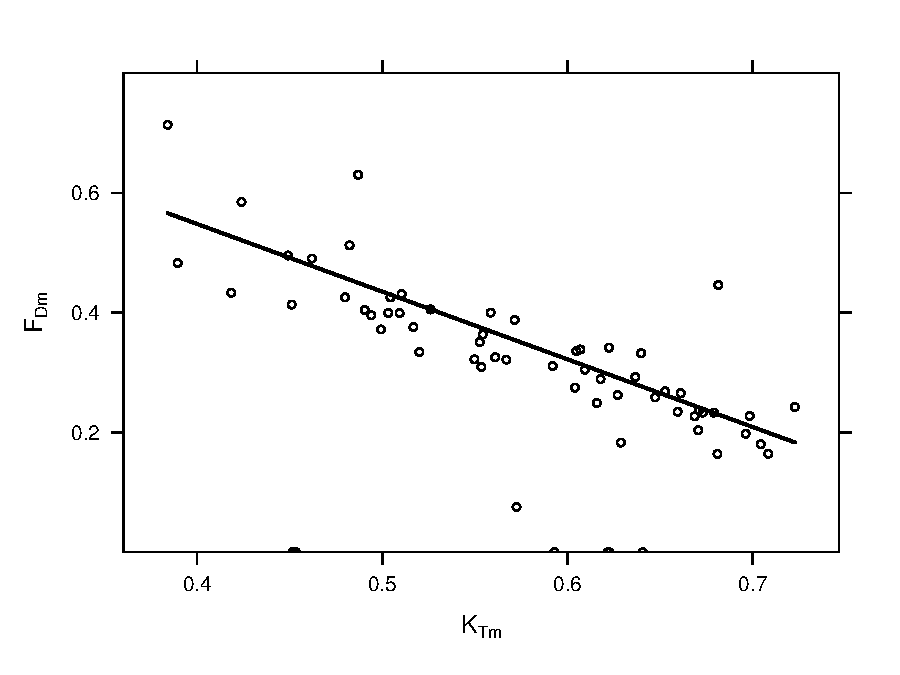
\includegraphics[scale=0.75]{../figs/FdKtMensual}

\caption{Correlación entre el índice de claridad y la fracción de difusa para
medias mensuales de valores diarios. Las medidas de radiación han
sido obtenidas de la base de datos HELIOS-IES (\protect\url{http://helios.ies-def.upm.es/}).\label{fig:KtmFDm}}

\end{figure}


Por ejemplo, un lugar que recibe en el plano horizontal $\SI{3150}{\Wh\per\meter\squared}$
de media mensual de irradiación global diaria en un mes que corresponde
a media mensual de irradiación extraterrestre diaria de $\SI{4320}{\Wh\per\meter\squared}$
tendrá, en ese mes, un índice de claridad mensual $K_{Tm}=\frac{3150}{4320}=0.73$
y, según la correlación de Page, una fracción de difusa $F_{Dm}=1-1.13\cdot0.73=0.175$.
Por tanto, la media mensual de radiación difusa diaria será $D_{d,m}(0)=0.175\cdot3150=\SI{551.6}{\Wh\per\meter\squared}$
y la radiación directa será $B_{d,m}(0)=3150-551.6=\SI{2598,4}{\Wh\per\meter\squared}$.

De la misma forma, se pueden establecer correlaciones entre valores
diarios del índice de claridad y la fracción de difusa. Sin embargo,
al disminuir la escala temporal la dispersión de valores aumenta sensiblemente
y así el error asociado a las regresiones propuestas. Más adelante
analizaremos la variabilidad de la radiación solar y su relación con
la escala temporal. Por ahora tendremos en cuenta este hecho para
manejar con precaución los resultados de las correlaciones para valores
diarios. A esta precaución añadimos que el verdadero interés de nuestro
análisis consiste en obtener información que nos permita estimar la
energía producida por un sistema fotovoltaico durante un período largo
(por ejemplo, un año). Como veremos en sucesivos capítulos, el funcionamiento
de un sistema fotovoltaico está determinado en primer lugar por la
radiación incidente, aunque existen otros factores de segundo orden
que no se pueden despreciar, principalmente la temperatura. Sin embargo,
las fluctuaciones de estos factores de segundo orden sufren una atenuación
considerable cuando el período de cálculo es suficientemente largo.
Recordando que Liu y Jordan comprobaron que las medias mensuales de
la radiación diaria caracterizaban su comportamiento durante ese mes,
concluimos que las estimaciones de energía producida pueden realizarse
con fiabilidad adecuada empleando las correlaciones para medias mensuales. 

Cuando sea necesario el cálculo de la radiación difusa en un día determinado,
es recomendable la correlación propuesta por Collares Pereira y Rabl
\cite{Collares-Pereira.Rabl1979}(Figura \ref{fig:KtFDd}):\begin{equation}
F_{Dd}=\begin{cases}
0.99 & K_{Td}\leq0.17\\
1.188-2.272\cdot K_{Td}+9.473\cdot K_{Td}^{2}-21.856\cdot K_{Td}^{3}+14.648\cdot K_{Td}^{4} & K_{Td}>0.17\end{cases}\label{eq:FDdCollares}\end{equation}
\nomenclature[Fdd]{$F_{Dd}$}{Fracción de difusa diario}

%
\begin{figure}
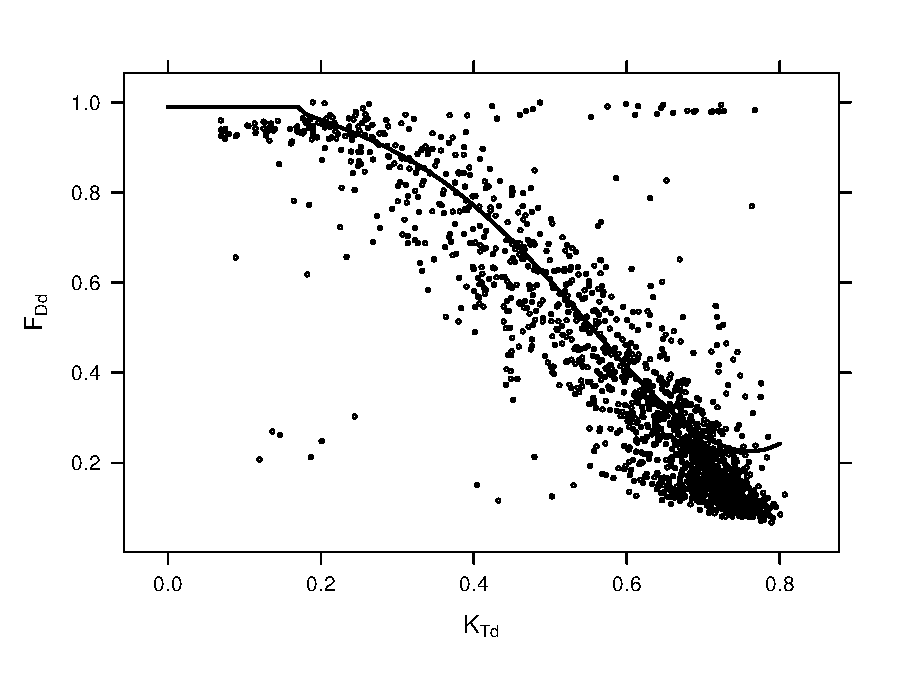
\includegraphics[scale=0.75]{../figs/FdKtDiario}

\caption{Correlación entre el índice de claridad y la fracción de difusa para
valores diarios. Las medidas de radiación han sido obtenidas de la
base de datos HELIOS-IES (\protect\url{http://helios.ies-def.upm.es/}).\label{fig:KtFDd}}

\end{figure}


En la escala temporal diaria, a pesar de que la definición del índice
de claridad permite atenuar la influencia de la latitud, los efectos
derivados de la climatología local se hacen más evidentes. De aquí
la existencia de una variedad muy amplia de correlaciones para valores
diarios (unas 250 publicadas según algunos autores \cite{Miguel.Bilbao.ea2001}),
muchas de las cuales aplican sólo a un lugar concreto. El lector interesado
puede consultar las siguientes referencias \cite{Miguel.Bilbao.ea2001,Soler1990,Gopinathan.Soler1995,Macagnan1993}.
Estos mismos comentarios son aplicables de forma aún más acentuada
a las correlaciones entre valores horarios, y como ejemplo se proponen
estas referencias\footnote{Implementadas en \texttt{solaR} \cite{Perpinan2012b}. Consulte \href{http://search.r-project.org/R/library/solaR/html/corrFdKt.html}{\texttt{corrFdKt}}.} \cite{Collares-Pereira.Rabl1979, Erbs.Klein.ea1982, Ridley.Boland.ea2010}.


\subsection{Datos de radiación}

Los datos de radiación disponibles en bases de datos proceden de medidas
realizadas por estaciones terrestres o estimadas a partir de imágenes
de satélite. Las estaciones terrestres suelen ser estaciones agroclimáticas
dedicadas a la medida de variables meteorológicas y climáticas orientadas
principalmente al sector agrícola. Uno de los instrumentos que incorporan
es el piranómetro, dispositivo capaz de medir la radiación global.
En casos excepcionales incluyen un pirheliómetro, dispositivo que
mide la radiación directa, o un piranómetro de difusa. La información
recogida por las redes de estaciones agroclimáticas suele estar disponible
en páginas de Internet. En el apéndice \ref{chap:enlaces} se incluye una
relación de estas páginas.

La cobertura espacial que ofrece la red de estaciones terrestres es
muy limitada por lo que frecuentemente hay que recurrir a interpolaciones
entre varias estaciones (aproximación válida sólo cuando existe una
distancia mínima) o a imágenes de satélite. Las imágenes procedentes
de satélites geoestacionarios meteorológicos (por ejemplo, el Meteosat)
pueden ser interpretadas para estimar la radiación incidente en la
superficie terrestre. Es necesario resaltar que el valor obtenido
es una medida indirecta a través de un algoritmo de análisis, con
el consiguiente error asociado. No obstante, su alta cobertura espacial
y disponibilidad han fomentado su uso en los últimos años. Existen
varias bases de datos disponibles en Internet, tales como las que se
incluyen en el apéndice \ref{chap:enlaces}.

Para la elección de la base de datos debe resolverse el compromiso
entre cercanía de la medida al lugar de la instalación y larga duración
de la base temporal. Debe tenerse en cuenta que las discrepancias
entre bases de datos pueden llegar a ser de hasta el 30\%, y por tanto,
todos los resultados posteriores deben manejarse sin perder la perspectiva
de esta incertidumbre. Por tanto, es sumamente importante referenciar
cualquier estimación de energía a la base de datos empleada para el
cálculo.

En cualquier caso, la información disponible en las bases de datos
suele estar limitada a valores diarios de radiación global en el plano
horizontal. A partir de esta información deberemos realizar un procedimiento
de cálculo para estimar el valor de la radiación difusa y directa,
y trasladar estos valores a los correspondientes en un plano inclinado.


\section{Radiación en superficies inclinadas}

El procedimiento de cálculo\footnote{Implementado en la función
  \href{http://search.r-project.org/R/library/solaR/html/calcGef.html}{\texttt{calcGef}}
  de \texttt{solaR} \cite{Perpinan2012b}} que debe recorrerse para obtener valores
de irradiación global en un plano inclinado a partir de valores de
irradiación global en el plano horizontal es el descrito en la figura
\ref{fig:Procedimiento-de-calculo}. Partiremos de valores de
irradiación global diaria en el plano horizontal. 
En el caso de disponer sólo de medias mensuales, se emplea la ecuación
\ref{eq:Page} para obtener las respectivas medias mensuales
de irradiación difusa y directa diaria en el plano
horizontal. Si la información disponible es una serie temporal de
valores diarios, la correlación definida por la ecuación
\ref{eq:FDdCollares} permite obtener los correspondientes valores
diarios de irradiación difusa y directa diaria en el plano horizontal.

A continuación, como paso intermedio para poder efectuar las transformaciones
al plano inclinado, estimaremos valores de irradiancia difusa,
directa y global en el plano horizontal.  Con estas estimaciones de irradiancia en el plano horizontal podremos calcular los valores correspondientes
en el plano del generador. 

Integrando los valores de irradiancia obtendremos
las estimaciones de irradiación diaria difusa, directa y global en
el plano del generador. El apellido de ``incidente'' indica que es
el resultado de tener en cuenta la inclinación y orientación del generador.
Sin embargo, para considerar también las pérdidas por suciedad, transmitancia
del vidrio del módulo y reflexión por incidencia no perpendicular,
deberemos realizar un paso adicional y añadir el apellido de ``efectiva''
a la irradiancia y a la irradiación. Será esta irradiación incidente
efectiva la que emplearemos en los cálculos de energía producida por
un sistema fotovoltaico. 

%
\begin{figure}
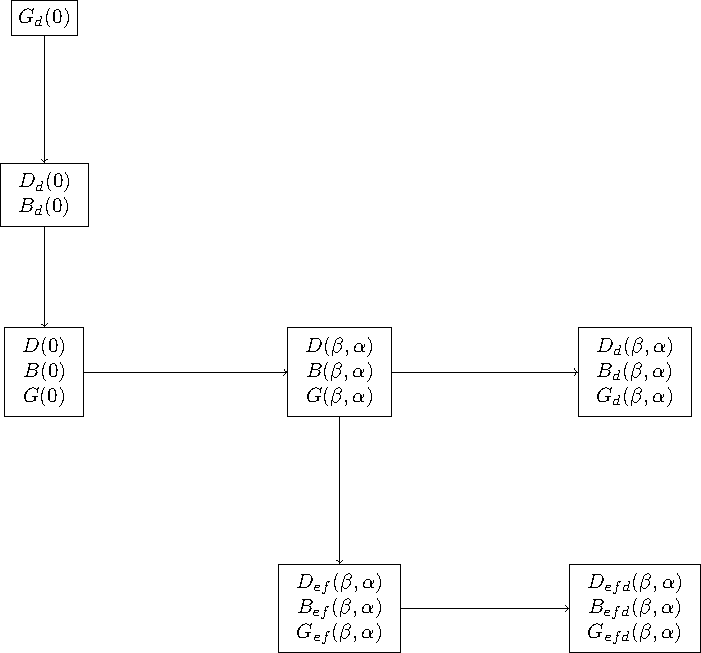
\includegraphics{../figs/ProcedimientoCalculoRadiacionInclinada}

\caption{Procedimiento de cálculo.\label{fig:Procedimiento-de-calculo}}

\end{figure}



\subsection{Estimación de irradiancia a partir de irradiación diaria}

Supongamos que disponemos de un conjunto de valores de irradiación diaria
difusa, directa y global en el plano horizontal. Para realizar la
transformación al plano inclinado es necesario estimar el perfil de
irradiancia correspondiente a cada valor de irradiación. Dado que
la variación solar durante una hora es baja, podemos suponer que el
valor medio de la irradiancia durante esa hora coincide numéricamente
con la irradiación horaria.%
\footnote{Es importante recordar que empleamos unidades de $\si{\kWh\per\meter\squared}$
para la irradiación y $\si{\kW\per\meter\squared}$ para la
irradiancia.}. 
Por otra parte, el análisis de valores \emph{medios} en \emph{largas}
series temporales ha mostrado que la relación entre la irradiancia
y la irradiación difusa es equivalente a la existente entre la irradiancia
y la irradiación extra-atmosférica \cite{Collares-Pereira.Rabl1979}
(ecuación \ref{eq:Rd}):

\begin{equation}
r_{D}=\frac{D(0)}{D_{d}(0)}=\frac{B_{o}(0)}{B_{0d}(0)}\label{eq:Rd}\end{equation}
\nomenclature[rd]{$r_{D}$}{Relación entre la irradiancia y la irradiación difusa en el plano horizontal}\nomenclature[rg]{$r_{G}$}{Relación entre la irradiancia y la irradiación global en el plano horizontal}

Este factor $r_{D}$ es calculable directamente sabiendo que la relación
entre irradiancia e irradiación extra-atmosférica es deducible teóricamente
a partir de las ecuaciones \ref{eq:Bo0} y \ref{eq:Bo0d}:

\begin{equation}
  \frac{B_{o}(0)}{B_{0d}(0)}=\frac{\pi}{T}\cdot\frac{\cos(\omega)-\cos(\omega_{s})}{\omega_{s}\cdot\cos(\omega_{s})-\sin(\omega_{s})}\label{eq:RelacionExtraAtmosferica}\end{equation}
donde $T$ es la duración del día en horas, $\omega_s$ está expresado en
radianes y $\omega$ corresponde
al instante central de la hora correspondiente.

El mismo análisis mostró una relación entre la irradiancia e irradiación
global asimilable a una función dependiente de la hora solar (ecuación
\ref{eq:Rg}):

\begin{equation}
r_{G}=\frac{G(0)}{G_{d}(0)}=r_{D}\cdot\left(a+b\cdot\cos(\omega)\right)\label{eq:Rg}\end{equation}
siendo

\begin{align}
a & =0.409-0.5016\cdot\sin(\omega_{s}+\frac{\pi}{3})\\
b & =0.6609+0.4767\cdot\sin(\omega_{s}+\frac{\pi}{3})
\end{align}
donde $\omega_s$ es negativa y está expresada en radianes.

Es importante resaltar que estos perfiles proceden de medias sobre
largos períodos, y de ahí que, como es observable en la figura \ref{fig:Perfil-de-irradiancia},
las fluctuaciones propias del movimiento de nubes a lo largo del día
queden atenuadas y se obtenga una curva sin alteraciones. Evidentemente,
las dos curvas encierran un área de valor unidad. La curva correspondiente
a la radiación global ($r_{G}$) es algo más estrecha y elevada que
la correspondiente a la difusa. Este hecho se explica teniendo en
cuenta que la masa de aire%
\footnote{Recordemos que la masa de aire es la relación entre caminos recorridos
por los rayos directos del Sol a través de la atmósfera. Dado que
la radiación global incluye la radiación directa, este efecto es apreciable
en su curva y no en la de la radiación difusa.%
} es mayor en el amanecer y atardecer que en el mediodía.


\begin{figure}
\begin{centering}
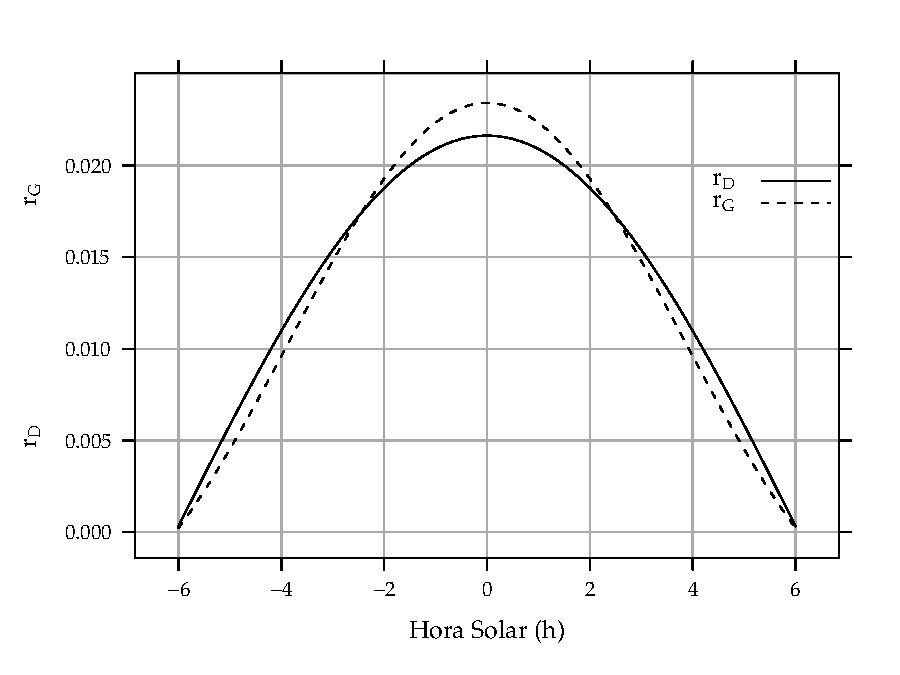
\includegraphics[scale=0.75]{../figs/RgRd}
\end{centering}

\caption{Perfil de irradiancia difusa y global obtenido a partir del generador
empírico de \cite{Collares-Pereira.Rabl1979} para valores de irradiancia
tomadas cada 10 minutos.\label{fig:Perfil-de-irradiancia} }

\end{figure}



\subsection{Transformación al plano del generador}

Una vez obtenidos los valores de irradiancia en el plano horizontal,
podemos estimar las componentes de irradiancia en el plano del
generador.  La irradiancia directa es calculable mediante criterios
puramente geométricos, teniendo en cuenta el ángulo cenital solar y el
ángulo de incidencia en el generador. Cuando el Sol se encuentra
detrás del plano del generador, el coseno del ángulo de incidencia es
negativo.  Por tanto, para no tomar en consideración la radiación
directa en estos instantes, sustituiremos este valor por cero:

\begin{align}
  B(\beta,\alpha) & =B(n) \cdot \max(0,\cos(\theta_{s}))\\
  & =B(0) \cdot \frac{\max(0,\cos(\theta_{s}))}{\cos(\theta_{zs})}
  \label{eq:DirectaPlanoGenerador}
\end{align}

donde se ha empleado la equivalencia $B(0) = B(n) \cdot
\cos(\theta_{zs})$


El cálculo de la radiación difusa es algo más complejo. Debe tomar en
consideración en cada instante las contribuciones de aquellos puntos
pertenecientes a la región de la esfera celeste que son visibles por
el generador. El tamaño de esta región depende de la inclinación del
generador, tal y como se muestra en la figura
\ref{fig:RegionVisibleCielo}.  La ecuación \ref{eq:DifusaIntegral} lo
expresa en lenguaje matemático, calculando la irradiancia difusa
integrando la radiancia%
\footnote{La radiancia, $L$, en una determinada dirección respecto a
  la normal a la superficie, $\theta$, se define como el flujo de
  densidad de potencia por unidad de ángulo sólido,
  $L=\frac{\Phi}{\mathrm{d}A\cdot\mathrm{d}\Omega\cdot\cos\theta}$ ,
  donde $\Phi$ representa el flujo de potencia, $\mathrm{d}A$ el
  diferencial de área de la fuente radiante, $\mathrm{d}\Omega$ el
  diferencial de ángulo sólido que contiene el cono de radiación. %
} en esta región visible (expresada en esta ecuación con el ángulo
sólido $\Omega$).

\begin{equation}
  D(\beta,\alpha)=\intop_{\Omega}L(\theta_{z},\psi)\cdot\cos(\theta_{z}^{'})d\Omega\label{eq:DifusaIntegral}\end{equation}
donde $\theta_{z}^{'}$ es el ángulo de incidencia entre el elemento
de integración y el plano del generador.

%
\begin{figure}
  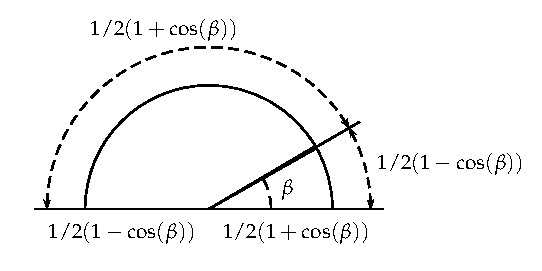
\includegraphics{../figs/AnguloVisionCielo}

  \caption{Ángulo de visión del cielo.\label{fig:RegionVisibleCielo}}

\end{figure}


La resolución de la ecuación \ref{eq:DifusaIntegral} es sumamente
compleja debido a que la distribución de la radiancia depende del
tamaño, posición, brillo y movimiento de las nubes. Para obtener
soluciones abordables es preciso realizar aproximaciones sobre este
comportamiento.  La primera consiste en suponer que la esfera celeste
es isotrópica y por tanto $L(\theta_{z},\psi)=\mathrm{cte}$. Con esta
aproximación, y teniendo en cuenta la figura
\ref{fig:RegionVisibleCielo} la irradiancia difusa sobre un plano
inclinado es:

\begin{equation}
  D(\beta,\alpha)=D(0)\cdot\frac{1+\cos(\beta)}{2}\label{eq:DifusaIsotropica}\end{equation}


Sin embargo, salvo días cubiertos, la esfera celeste no es uniforme,
sino que la radiancia difusa es máxima en las cercanías al Sol (región
circunsolar). Al no considerar de forma especial esta región, esta
aproximación simple subestima los valores que se pueden recibir en
planos que miran al ecuador y, por tanto, orientados hacia esta región
circunsolar. Los modelos anisotrópicos toman en consideración esta
distribución y ponderan las contribuciones de la región circunsolar y
el resto de la esfera celeste. Es destacable la propuesta de
\cite{Hay.McKay1985} (ecuación \ref{eq:DifusaHay}). Estos autores
proponen tratar la radiación procedente de la región circunsolar como
si fuese radiación directa (ecuación \ref{eq:DifusaCircumsolar}) y el
resto de la esfera celeste como isotrópica (ecuación
\ref{eq:DifusaIsotropicaHay})\footnote{Es posible mejorar este modelo
  para tener en cuenta que el horizonte es más brillante que el resto
  del cielo, incluyendo un factor de modulación como el propuesto en
  \cite{Reindl.Beckman.ea1990}}.  La proporción entre las dos
regiones se estima con el índice de anisotropía, $k_{1}$, como la
relación entre la irradiancia directa y la irradiancia
extra-atmosférica, ambas en el plano horizontal
(\ref{eq:AnisotropiaHay}\nomenclature[k1]{$k_{1}$}{Índice de
  anisotropía}).  Así, cielos muy cubiertos conducen a valores bajos
del índice de anisotropía, de forma que casi toda la radiación difusa
será isotrópica. Sin embargo, con cielos claros el índice de
anisotropía será elevado y la contribución de la región circunsolar
aumentará.

\begin{align}
  D(\beta,\alpha) & =D^{I}(\beta,\alpha)+D^{C}(\beta,\alpha)\label{eq:DifusaHay}\\
  D^{I}(\beta,\alpha) & =D(0)\cdot(1-k_{1})\cdot\frac{1+\cos(\beta)}{2}\label{eq:DifusaIsotropicaHay}\\
  D^{C}(\beta,\alpha) & =D(0)\cdot k_{1}\cdot\frac{\max(0,\cos(\theta_{s}))}{\cos(\theta_{zs})}\label{eq:DifusaCircumsolar}\\
  k_{1} & =\frac{B(n)}{B_{0}\cdot\epsilon_0} = \frac{B(0)}{B_{0}(0)}\label{eq:AnisotropiaHay}
\end{align}
\nomenclature[Di]{$D_{I}$}{Irradiancia difusa isotrópica}
\nomenclature[Dc]{$D_{C}$}{Irradiancia difusa circumsolar}

La irradiancia de albedo suele considerarse como isotrópica. Esta
aproximación es aceptable para esta componente debido a su baja
contribución a la radiación global. Comúnmente se calcula a partir de
la irradiancia global en el plano horizontal con un coeficiente de
reflexión, $\rho$, cuyo valor depende de las características del
terreno. Si no existe información disponible para calcularlo un valor
de $\rho=0.2$\nomenclature[rho]{$\rho$}{Coeficiente de reflexión del
  terreno para la irradiancia de albedo} es aceptable para un terreno
normal. En la ecuación \ref{eq:Albedo} utilizamos el factor
$\frac{1-\cos(\beta)}{2}$, complementario del factor de visión
correspondiente a la difusa isotrópica.

\begin{equation}
  R(\beta,\alpha)=\rho\cdot G(0)\cdot\frac{1-\cos(\beta)}{2}\label{eq:Albedo}\end{equation}



\section{Incertidumbre}

Una vez obtenidos los valores de irradiancia sobre un plano inclinado,
es posible realizar el cálculo de la irradiación diaria, mensual o
anual sobre un plano cualquiera. Estas estimaciones son frecuentemente
empleadas para responder a preguntas tales como {}``¿Cuánta energía
producirá este sistema?''. La respuesta a este tipo de preguntas
conlleva realizar un ejercicio de predicción con una incertidumbre
asociada. La amplitud de la incertidumbre depende de la varianza de
la variable aleatoria en estudio (la producción de un sistema fotovoltaico)
y del tipo de predicción deseada. 

Analicemos en primer lugar la varianza de la variable aleatoria. Supongamos
primero que la distribución que caracteriza a la variable aleatoria
es asimilable a una gaussiana. En este caso sabemos que, para obtener
una confianza del 95\% en nuestra predicción, deberemos admitir un
intervalo acotado por $1.96\cdot\sigma_{X}$ , donde $\sigma_{X}$
es la desviación estándar de la variable aleatoria gaussiana $X$.
¿Qué valores toma esta desviación cuando nuestra variable aleatoria
es la radiación global?

Por comodidad, utilicemos la variabilidad interanual o incertidumbre
relativa de una variable aleatoria $X$, que se puede calcular con
su desviación estándar y su media: $\delta_{X}=\sigma_{X}/\overline{X}$,
Analicemos la variabilidad para períodos diarios ($\sigma_{G0d}/\overline{G_{d}(0)}$)
, mensuales ($\sigma_{G0m}/\overline{G_{m}(0)}$) y anuales ($\sigma_{G0y}/\overline{G_{y}(0)}$)
de la irradiación global horizontal. Para este análisis emplearemos
un conjunto de valores procedentes de la estación meteorológica de
Carmona-Tomejil (Andalucía). Este conjunto de datos abarca el período
comprendido entre Septiembre de 2001 y Septiembre de 2008. en la figura
\ref{fig:VariabilityRadiation} se recoge la evolución de la variabilidad
diaria para cada día del año, la variabilidad mensual para cada mes
y la evolución temporal de la irradiación anual para los años 2001
a 2007.

%
\begin{figure}
\begin{centering}
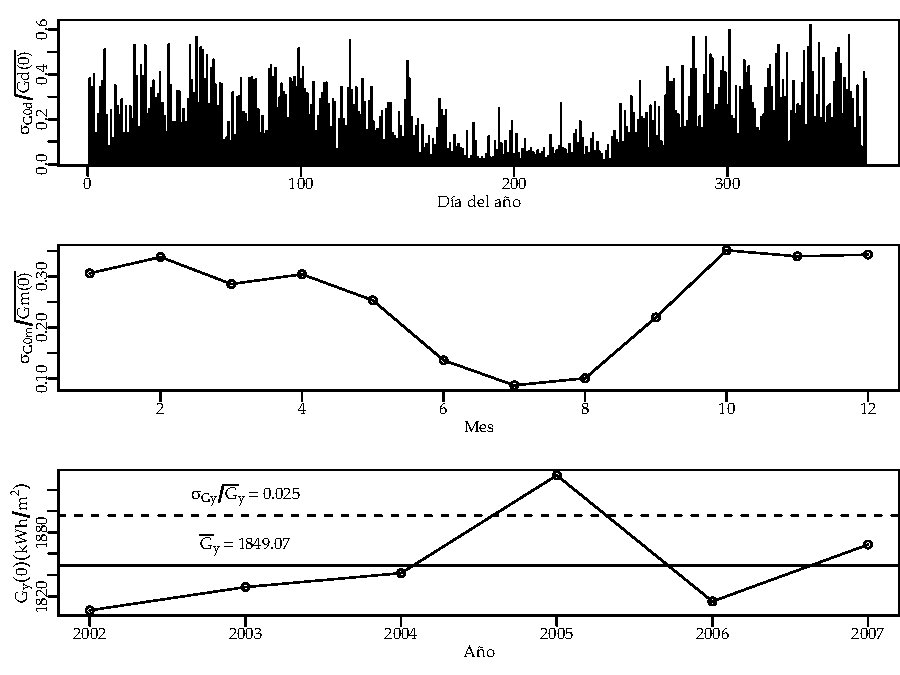
\includegraphics[scale=0.75]{../figs/VariabilidadRadiacionDiario}
\end{centering}

\caption{\label{fig:VariabilityRadiation}Variabilidad de la irradiación diaria,
mensual y anual durante el período comprendido entre 2001-2008.}

\end{figure}


La variabilidad diaria oscila entre 0.6 para el invierno y 0.1 para
el verano. Los valores mensuales oscilan entre el 0.35 para el invierno
y 0.1 para el verano. La variabilidad anual es del 2.5\%. Estos resultados
son similares a los publicados por PVGIS \cite{Suri.Huld.ea2007}.

Para analizar la variabilidad de la irradiación en el plano inclinado,
tengamos en cuenta que ésta es una función de la irradiación horizontal,
y por tanto su variabilidad puede ser derivada mediante la teoría
de la propagación del error \cite{Navidi2008}:

\begin{equation}
\delta_{G_{ef}}=\frac{\overline{G(0)}}{\overline{G(I)}}\cdot\left|\frac{dG(I)}{dG(0)}\right|\cdot\delta_{G(0)}\end{equation}


Es posible mostrar \cite{Perpinan2009} que, para sistemas de seguimiento
a doble eje, el valor absoluto de la derivada es mayor que la unidad
durante todo el período estudiado. De esta forma, la variabilidad
de la irradiación incidente es superior al de la irradiación horizontal.
 Para sistemas estáticos la derivada es mayor que la unidad durante
casi todo el período, lo que indica que, aunque con menor intensidad
que en sistemas de doble eje, también la variabilidad de la irradiación
incidente que incide en un plano estático es superior a la de la irradiación
horizontal.

Volvamos al ejercicio de predicción que enunciábamos al comienzo de
esta sección. Ahora vemos que la predicción para una fecha concreta
lleva asociada una incertidumbre variable según la época del año,
pero en todo caso elevada. Cuando nos conformamos con saber lo que
ocurrirá durante un mes determinado de un año concreto, reduciremos
la incertidumbre, pero aún así los valores serán altos. Ahora bien,
si extendemos la predicción a todo el ciclo de vida y nos conformamos
con saber lo que ocurrirá en promedio, la teoría estadística muestra
que la desviación estándar asociada (denominada desviación estándar
de la media) es sustancialmente inferior, según la relación $\sigma_{\bar{X}}=\frac{\sigma_{X}}{\sqrt{N}}$,
donde N es el número de años al que extendemos la predicción%
\footnote{En sentido estricto, esta relación es aplicable sólo si la serie temporal
sobre la que se ha calculado la desviación estándar es suficientemente
amplia para considerar que caracteriza a los valores futuros. Dicho
en lenguaje estadístico, la longitud de la muestra debe garantizar
que su desviación estándar es equivalente a la de la población.%
}. Por ejemplo, si hacemos una predicción para conocer el comportamiento
promedio durante 25 años, dividimos por 5 la desviación estándar asociada,
y por tanto, obtendremos estimaciones cuya incertidumbre suficientemente
baja para ser útil. 

Sinteticemos este apartado afirmando que la radiación, como proceso
estocástico, lleva asociada una incertidumbre que debe ser considerada
al emplear las estimaciones de los apartados anteriores. Esta incertidumbre
es mayor cuánto menor es el período de cálculo y más apreciable en
el invierno que en el verano. El paso a la radiación en el plano inclinado
aumenta la incertidumbre, agravando el problema. Lo razonable en este
contexto es realizar predicciones del comportamiento promedio durante
un período prolongado de tiempo, y descartar las predicciones para
una fecha concreta.


\section{Ángulo de Incidencia y Suciedad\label{sec:RadiacionEfectiva}}

Salvo en sistemas de seguimiento, la radiación incidente en un módulo
fotovoltaico está frecuentemente desviada de la normal a la superficie
del módulo. Esta desviación, cuantificada con el ángulo de incidencia,
$\theta_{s}$ (por ejemplo, ecuación \ref{eq:cosThetaEstatica} para
un sistema estático), es causa de pérdidas por reflexión, también
denominadas pérdidas angulares. Además, la suciedad acumulada en la
superficie del módulo altera las propiedades angulares del mismo y
reduce la transmitancia del vidrio (representada por $T_{limpio}(0)$\nomenclature[Tlimpio]{$T_{limpio}(0)$}{Transmitancia de un vidrio limpio}\nomenclature[Tsucio]{$T_{sucio}(0)$}{Transmitancia de un vidrio sucio}
cuando el módulo está limpio). Estos dos fenómenos reducen la irradiancia
que es aprovechable por el módulo, a la que añadiremos el apellido
de {}``efectiva''. Para el caso de radiación directa, la expresión
de irradiancia efectiva queda recogida en la ecuación \ref{eq:Bef}:

\begin{equation}
B_{ef}(\beta,\alpha)=B(\beta,\alpha)\cdot\left[\frac{T_{sucio}(0)}{T_{limpio}(0)}\right]\cdot(1-FT_{B}(\theta_{s}))\label{eq:Bef}\end{equation}
donde $FT_{B}(\theta_{s})$\nomenclature[FTb]{$FT_{B}$}{Factor de pérdidas angulares para la irradiancia directa}
es el factor de pérdidas angulares para la irradiancia directa, calculable
mediante la ecuación\footnote{Implementada en las funciones
  \href{http://search.r-project.org/R/library/solaR/html/fInclin.html}{\texttt{fInclin}}
  y
  \href{http://search.r-project.org/R/library/solaR/html/calcGef.html}{\texttt{calcGef}}
  de \texttt{solaR} \cite{Perpinan2012b}} \ref{eq:FTb} \cite{Martin.Ruiz2001}: 
\begin{equation}
FT_{B}(\theta_{s})=\frac{\exp(-\frac{\cos(\theta_{s})}{a_{r}})-\exp(-\frac{1}{a_{r}})}{1-\exp(-\frac{1}{a_{r}})}
\label{eq:FTb}
\end{equation}


Este factor depende del ángulo de incidencia y del coeficiente de
pérdidas angulares, $a_{r}$. Es sencillo comprobar que cuando la
radiación es perpendicular a la superficie ($\theta_{s}=0$), el valor
de $FT_{B}$ es cero. En la figura \ref{fig:PerdidasAngulares} comprobamos
que las pérdidas angulares sólo son apreciables a partir de desviaciones
superiores a los $\ang{60}$, acentuándose para suciedades crecientes.
Así, observamos que el ángulo de visión de un módulo plano convencional
es muy amplio o, en otras palabras, la sensibilidad a la desorientación
de un módulo plano es muy baja. Tomaremos nuevamente en consideración
este hecho cuando analicemos la productividad asociada a la inclinación
y orientación de un sistema fotovoltaico de conexión a red (sección
\ref{sub:Orientacion-e-inclinacion}).

%
\begin{figure}
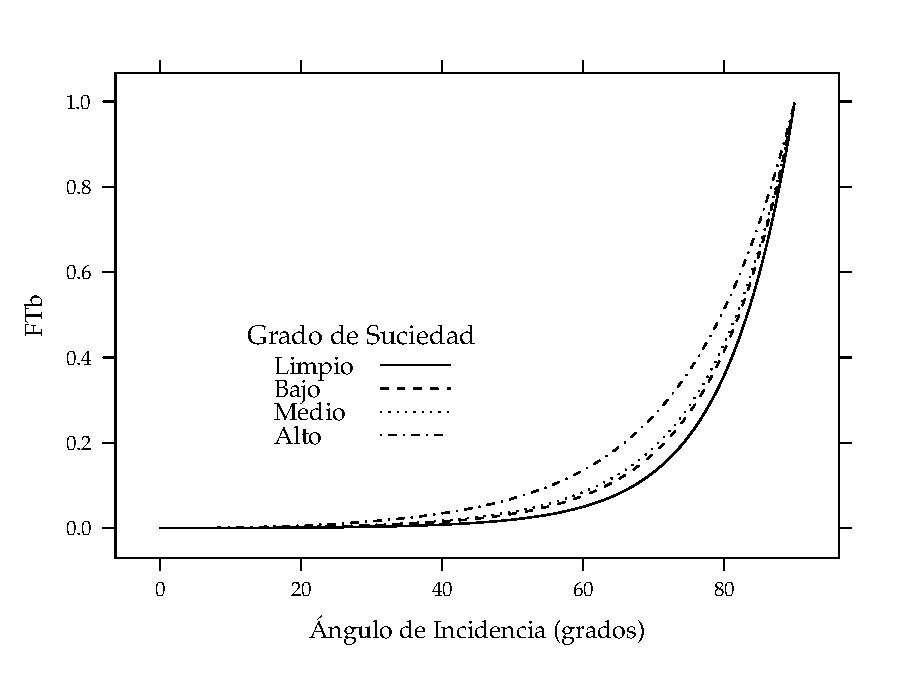
\includegraphics[scale=0.7]{../figs/Suciedad}

\caption{Pérdidas angulares de un módulo fotovoltaico para diferentes grados
de suciedad en función del ángulo de incidencia.\label{fig:PerdidasAngulares} }

\end{figure}


Los valores del coeficiente de pérdidas angulares deben ser determinados
de forma experimental. En la tabla \ref{tab:ar}quedan recogidos algunos
valores característicos de un módulo de silicio monocristalino convencional
para diferentes grados de suciedad. En esta tabla también se recogen
los valores de la transmitancia al interior del módulo en incidencia
normal respecto a la de un módulo limpio, $\frac{T_{sucio}(0)}{T_{limpio}(0)}$.

%
\begin{table}
\caption{Valores del coeficiente de pérdidas angulares y transmitancia relativa
en incidencia normal para diferentes tipos de suciedad.\label{tab:ar}}


\begin{tabular}{cccc}
\toprule 
Grado de Suciedad & $\frac{T_{sucio}(0)}{T_{limpio}(0)}$ & $a_{r}$ & $c_{2}$\tabularnewline
\midrule
\midrule 
Limpio & 1 & 0.17 & -0.069\tabularnewline
\midrule 
Bajo & 0.98 & 0.20 & -0.054\tabularnewline
\midrule 
Medio & 0.97 & 0.21 & -0.049\tabularnewline
\midrule 
Alto & 0.92 & 0.27 & -0.023\tabularnewline
\bottomrule
\end{tabular}
\end{table}


Para las componentes difusa isotrópica y de albedo existen otras
expresiones\footnote{Implementadas en las funciones
  \href{http://search.r-project.org/R/library/solaR/html/fInclin.html}{\texttt{fInclin}}
  y
  \href{http://search.r-project.org/R/library/solaR/html/calcGef.html}{\texttt{calcGef}}
  de \texttt{solaR} \cite{Perpinan2012b}}
(ecuaciones \ref{eq:FTd} y \ref{eq:FTr}) que dependen del ángulo
de inclinación del generador, del coeficiente de pérdidas angulares
y de dos coeficientes de ajuste, $c_{1}$y $c_{2}$. El primero de
ellos toma el valor constante $c_{1}=\frac{4}{3\pi}$. Los valores
del segundo dependen linealmente de $a_{r}$, y quedan recogidos en
la tabla \ref{tab:ar}. En estas expresiones el ángulo $\beta$ está
en radianes.

\begin{eqnarray}
FT_{D}(\beta) & \simeq & \exp[-\frac{1}{a_{r}}\cdot(c_{1}\cdot(\sin\beta+\frac{\pi-\beta-\sin\beta}{1+\cos\beta})+c_{2}\cdot(\sin\beta+\frac{\pi-\beta-\sin\beta}{1+\cos\beta})^{2})]\label{eq:FTd}\\
FT_{R}(\beta) & \simeq & \exp[-\frac{1}{a_{r}}\cdot(c_{1}\cdot(\sin\beta+\frac{\beta-\sin\beta}{1-\cos\beta})+c_{2}\cdot(\sin\beta+\frac{\beta-\sin\beta}{1-\cos\beta})^{2})]\label{eq:FTr}\end{eqnarray}
\nomenclature[FTd]{$FT_{D}$}{Factor de pérdidas angulares para la irradiancia difusa}\nomenclature[FTr]{$FT_{R}$}{Factor de pérdidas angulares para la irradiancia de albedo}

Para estas componentes el cálculo de irradiancia efectiva es similar
al de la irradiancia directa (ecuaciones \ref{eq:Disoef} y \ref{eq:Ref}).
Para la componente difusa circunsolar emplearemos el factor de pérdidas
angulares de la irradiancia efectiva (ecuación \ref{eq:Dciref}):

\begin{eqnarray}
D_{ef}^{I}(\beta,\alpha) & = & D^{I}(\beta,\alpha)\cdot\left[\frac{T_{sucio}(0)}{T_{limpio}(0)}\right]\cdot(1-FT_{D}(\beta))\label{eq:Disoef}\\
D_{ef}^{C}(\beta,\alpha) & = & D^{C}(\beta,\alpha)\cdot\left[\frac{T_{sucio}(0)}{T_{limpio}(0)}\right]\cdot(1-FT_{B}(\theta_{s}))\label{eq:Dciref}\\
R_{ef}(\beta,\alpha) & = & R(\beta,\alpha)\cdot\left[\frac{T_{sucio}(0)}{T_{limpio}(0)}\right]\cdot(1-FT_{R}(\beta))\label{eq:Ref}\end{eqnarray}


Siguiendo el esquema de la figura \ref{fig:Procedimiento-de-calculo},
a partir de estas irradiancias efectivas se puede calcular el valor
de irradiación global efectiva diaria, mensual y anual. Una comparación
entre la irradiación global incidente y la efectiva permite comprobar
la influencia de la suciedad y el desapuntamiento en períodos temporales
largos. En la figura \ref{fig:PerdidasSuciedadReflexion} se representa
esta comparación en términos de irradiación anual, particularizada
para Madrid y un grado de suciedad medio, y para diferentes valores
de inclinación y orientación. De esta figura extraemos valores que
oscilan entre el 7\% y el 10\% según sea la inclinación y orientación
del generador estático.

%
\begin{figure}
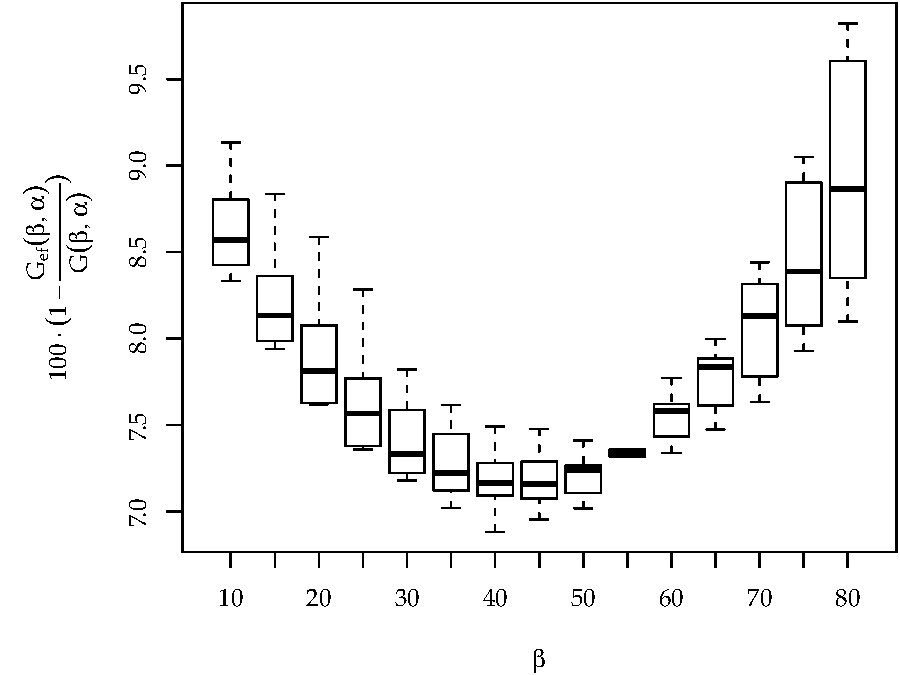
\includegraphics[scale=0.75]{../figs/GefVSG}

\caption{Pérdidas por suciedad e incidencia no perpendicular integradas a lo
largo de un año en Madrid, para un grado de suciedad medio, y para
diferentes ángulos de inclinación y orientación.\label{fig:PerdidasSuciedadReflexion}}

\end{figure}
\section{Aplicación práctica: cálculo para sistemas estáticos}

Una de las aplicaciones más comunes de la energía solar fotovoltaica
es la producción de energía eléctrica para su inyección en la red
eléctrica convencional. Estos sistemas, denominados sistemas fotovoltaicos
de conexión a red (capítulo \ref{cha:SFCR}), pueden emplear sistemas
de seguimiento para maximizar la producción o bien optar por estructuras
estáticas para reducir costes y ocupación de terreno. Analizaremos
la radiación incidente en sistemas estáticos durante un período anual.


\subsection{Inclinación óptima}

En estos casos, una de las preguntas a resolver es: suponiendo una
orientación hacia el ecuador, ¿qué inclinación es la adecuada para
conseguir la mayor producción eléctrica? Para resolver este problema
es importante resaltar que el objetivo de estos sistemas es obtener
la mayor producción \emph{anual}. 

% Según los conceptos de geometría solar expuestos, una superficie cuya
% inclinación sea igual a la latitud será paralela al eje de rotación
% terrestre. De esta forma, en los equinoccios será perpendicular al
% vector solar. Si no existiese atmósfera, la radiación que recibiría
% una superficie así inclinada sería la misma para cualquier latitud.
% Esta propiedad también se cumple en aquellas superficies que mantienen
% constante un determinado ángulo con la latitud . Es decir, si $\Delta=\beta-|\phi|$
% , todas aquellas superficies que mantengan $\Delta$ invariable recibirán
% la misma radiación para cualquier latitud en ausencia de atmósfera.
% Esta propiedad no es extensible a otros momentos del año porque la
% duración del día y el valor de la irradiación extra-atmosférica dependen
% de la latitud. Sin embargo, en un período \emph{anual} las variaciones
% entre el verano y el invierno se cancelan de forma que podríamos definir
% una función universal, valida para cualquier latitud, al modo de la
% ecuación \ref{eq:B_FuncionUniversal}:

% \begin{equation}
% \frac{B_{0d,a}(\beta)}{B_{0d,a}(\left|\phi\right|)}=f(\beta-\left|\phi\right|)\label{eq:B_FuncionUniversal}\end{equation}


% Esta función no es aplicable de forma directa cuando tomamos en consideración
% la interacción con la atmósfera, cuya composición y comportamiento
% varía con el lugar en cuestión. No obstante, es posible mostrar \cite{Lorenzo2006c}
% que cuando $\Delta=\beta-|\phi|$ toma valores entre $\ang{-20}$
% y $\ang{10}$ la influencia de la radiación de difusa no es importante,
% y por tanto aún podemos encontrar una función universal para la radiación
% global (ecuación \ref{eq:G_FuncionUniversal}):

% \begin{equation}
% \frac{G_{d,a}(\beta)}{G_{d,a}(\left|\phi\right|)}\approx f(\beta-\left|\phi\right|)\label{eq:G_FuncionUniversal}\end{equation}


Será necesario realizar los correspondientes cálculos de irradiación
global incidente con diversas inclinaciones. Del análisis de las curvas
correspondientes es posible obtener una relación que ligue la latitud
con el ángulo de inclinación que maximiza la producción\emph{ anual
}de un sistema fotovoltaico. En \cite{Lorenzo2006c} se propone la
siguiente relación entre el ángulo de inclinación y la latitud (ambos
en grados): \begin{equation}
\beta_{opt}=3.7+0.69\cdot|\phi|\label{eq:BetaOptimo}\end{equation}


Debido a la baja sensibilidad que los módulos planos tienen al desapuntamiento,
las pérdidas energéticas que obtendremos si no escogemos exactamente
el ángulo que resulta de la ecuación \ref{eq:BetaOptimo} serán muy
bajas. En la figura \ref{fig:PerdidasInclinacionOptima} observamos
que es necesario alejarse casi $\ang{10}$ del ángulo óptimo para
obtener unas pérdidas del 1\%.

%
\begin{figure}
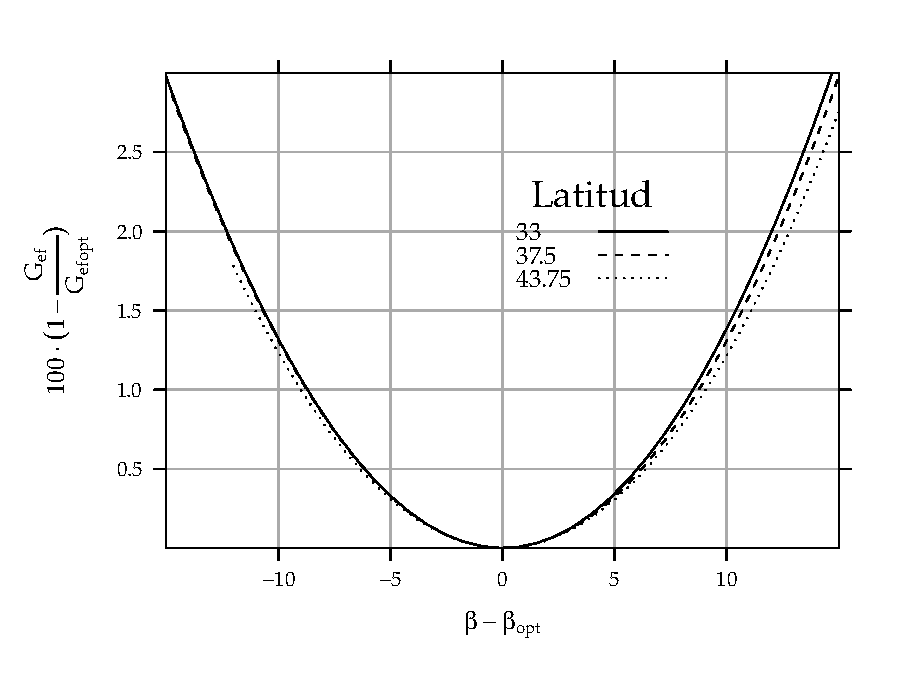
\includegraphics[scale=0.75]{../figs/PerdidasInclinacionOptima}

\caption{Pérdidas de irradiación global anual al elegir un ángulo de inclinación
diferente del óptimo para tres latitudes diferentes en el hemisferio
Norte.\label{fig:PerdidasInclinacionOptima}}



\end{figure}


Con este mismo análisis es posible relacionar la irradiación anual
para el ángulo óptimo de inclinación, $\beta_{opt}$, con la irradiación
anual en el plano horizontal , donde $\beta_{opt}$ está en grados
\cite{Caamano1998,Lorenzo2006c}:\nomenclature[Ga]{$G_{a}$}{Irradiación global anual}

\begin{equation}
\frac{G_{a}(0)}{G_{a}(\beta_{opt})}=1-4.46\cdot10^{-4}\cdot\beta_{opt}-1.19\cdot10^{-4}\cdot\beta_{opt}^{2}
\label{eq:GbetaOpt}
\end{equation}



\subsection{Irradiación anual efectiva}

Siguiendo este mismo camino es posible ajustar mediante regresiones
las curvas que relacionan la irradiación anual global efectiva con
la irradiación anual global incidente para sistemas estáticos. Dicho
de otra forma, podemos obtener regresiones que cuantifican las pérdidas
angulares y pérdidas por suciedad en términos anuales para sistemas
estáticos. Por ejemplo, en las referencias \cite{Caamano1998,Lorenzo2002}
se proponen las siguientes ecuaciones:

\begin{eqnarray}
\frac{G_{efa}(\beta,\alpha)}{G_{a}(\beta_{opt})} & = & g_{1}\cdot(\beta-\beta_{opt})^{2}+g_{2}\cdot(\beta-\beta_{opt})+g_{3}\label{eq:Gef_estefania}\\
g_{i} & = & g_{i1}|\alpha|^{2}+g_{i2}|\alpha|+g_{i3}\label{eq:Gef_estefania_coef}\end{eqnarray}
donde los ángulos $\beta_{opt}$, $\beta$ y $\alpha$ están en grados.

Los coeficientes para resolver las ecuaciones \ref{eq:Gef_estefania}
y \ref{eq:Gef_estefania_coef} son los recogidos en la tabla \ref{tab:CoefGef}
para el caso de un módulo con suciedad media ( $\frac{T_{sucio}(0)}{T_{limpio}(0)}=0.97$
).


\begin{table}
\begin{centering}
\begin{tabular}{cccc}
\toprule 
 & $i=1$ & $i=2$ & $i=3$\tabularnewline
\midrule
\midrule 
$g_{1i}$ & $8\cdot10^{-9}$ & $3.8\cdot10^{-7}$ & $-1.218\cdot10^{-4}$\tabularnewline
\midrule 
$g_{2i}$ & $-4.27\cdot10^{-7}$ & $8.2\cdot10^{-6}$ & $2.892\cdot10^{-4}$\tabularnewline
\midrule 
$g_{3i}$ & $-2.5\cdot10^{-5}$ & $-1.034\cdot10^{-4}$ & $0.9314$\tabularnewline
\bottomrule
\end{tabular}
\par\end{centering}

\caption{Valores de los coeficientes de la ecuación \ref{eq:Gef_estefania_coef}
necesarios para resolver la ecuación \ref{eq:Gef_estefania} para
el caso de un módulo con suciedad media.\label{tab:CoefGef}}

\end{table}

\section{Comparación entre Sistemas de Seguimiento}
\label{sec:comparacion-sistemas}

La sección \ref{sec:geometria-sistemas} detalla las ecuaciones que
rigen la geometría de la radiación incidente en sistemas estáticos y
de seguimiento. En esta sección aplicaremos esas ecuaciones al cálculo
de la radiación efectiva incidente en un generador. El lector
interesado puede consultar la referencia
\cite{Antonanzas-Torres.Canizares.ea2013}. En este documento se
detalla el cálculo de radiación efectiva para sistemas estáticos, con
seguimiento de eje horizontal Norte-Sur y sistemas de seguimiento de
doble eje usando datos de estaciones meteorológicas de la red
SIAR\cite{SIAR2011} y estimaciones a partir de imágenes de satélite
proporcionadas por el servicio CM~SAF\cite{CMSAF2011}.

Las figuras \ref{fig:MapasRadiacion}, \ref{fig:ComparativaRadiación} y
\ref{fig:HistComparativaRadiación} adaptadas del documento citado,
muestran que el seguimiento a doble eje es claramente más eficiente
para entregar radiación efectiva al generador que las otras dos
tecnologías, con incrementos que varían con la latitud y con la
radiación global anual en el plano horizontal. En relación con un
sistema estático, la mejora en radiación oscila entre el 10\% y 50\%,
siendo mejor para bajas latitudes y alta radiación. Comparado con el
seguimiento horizontal, la mejora se mueve en un margen estrecho
comprendido entre el 10\% y 15\%, con una relación poco clara con la
latitud y la radiación global en el plano horizontal.  La comparación
entre los sistemas estáticos y el seguimiento horizontal arroja
incrementos de radiación que oscilan entre el 5\% y 35\%, siendo
preferible el seguimiento horizontal para bajas latitudes y alta
radiación. Estas cifras deben tomarse como indicativas, teniendo en
cuenta la incertidumbre de los datos (base de datos de radiación,
correlaciones de radiación difusa, etc.) sobre los que se construyen
los mapas.

%
\begin{figure}
  \begin{centering}
    \subfloat[\label{fig:GefFixed}Sistema Estático.]{%
      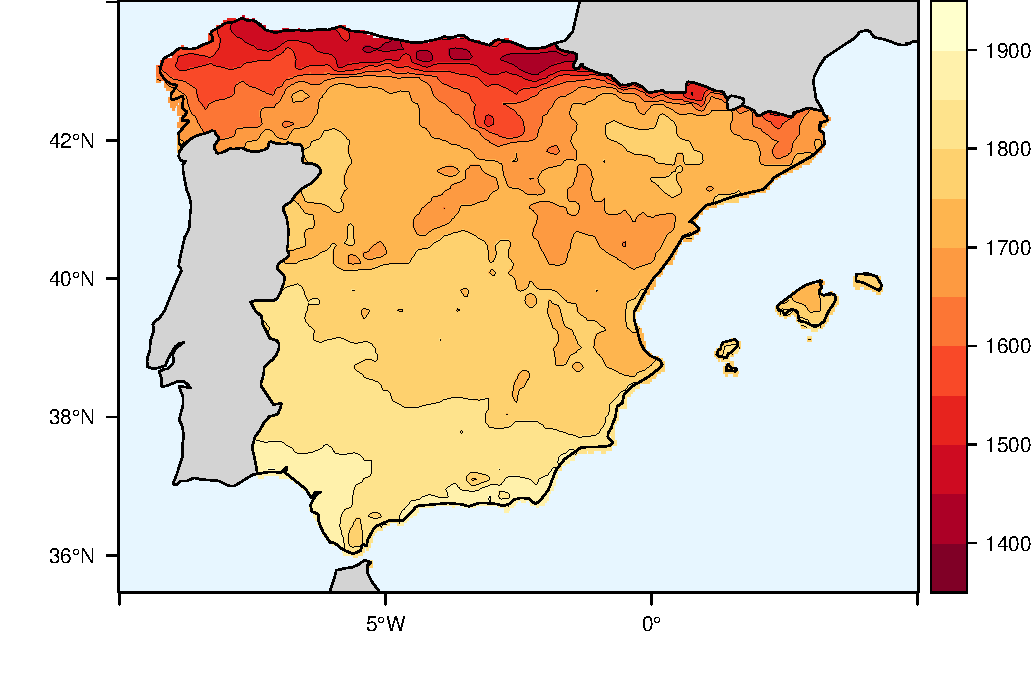
\includegraphics[height=0.3\textheight]{../figs/FixedKrig}
    }
  \end{centering}

\begin{centering}
  \subfloat[\label{fig:GefHorizNS}Seguimiento de eje horizontal
  N-S.]{%
    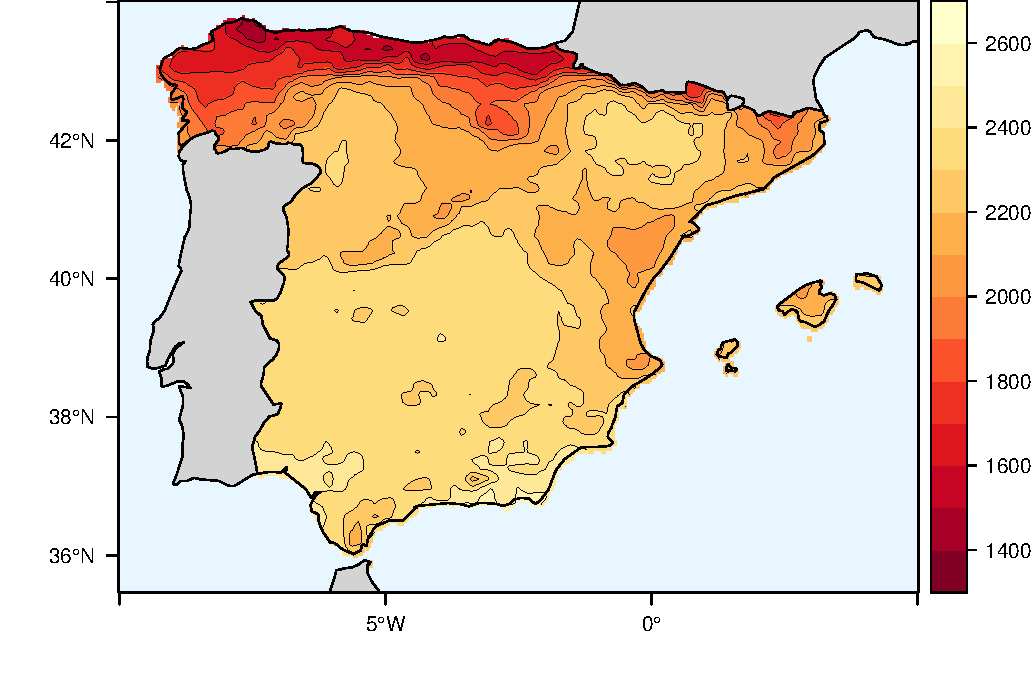
\includegraphics[height=0.3\textheight]{../figs/HorizKrig}
  }
  \par\end{centering}

\begin{centering}
  \subfloat[\label{fig:Gef2x}Seguimiento a doble eje.]{%
    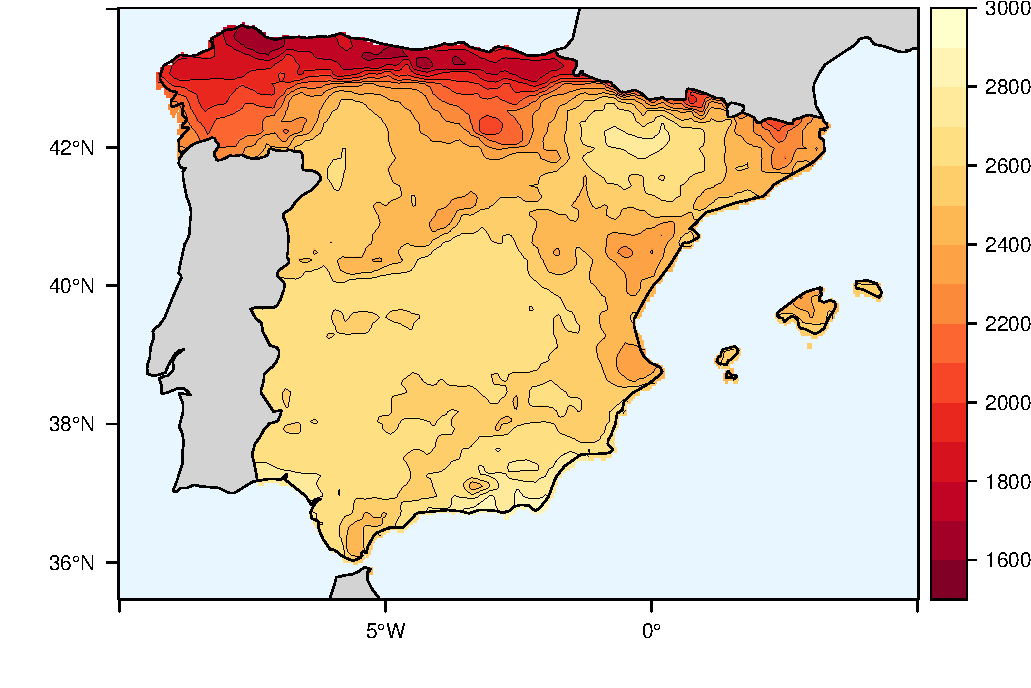
\includegraphics[height=0.3\textheight]{../figs/TwoKrig}
  }
  \par\end{centering}
\caption[Mapas de Radiación Efectiva]{Radiación Efectiva
  anual($\si{\kilo\Wh\per\squared\meter}$) recibida por sistemas
  estáticos, por sistemas de seguimiento con eje horizontal Norte-Sur
  y con seguimiento a doble eje. Los cálculos han sido realizados a
  partir de las bases de radiación SIAR \cite{SIAR2011} y CM~SAF
  \cite{CMSAF2011} según se detalla en
  \cite{Antonanzas-Torres.Canizares.ea2013}.}
\label{fig:MapasRadiacion}
\end{figure}


%
\begin{figure}
  \begin{centering}
    \subfloat[Doble eje frente a Estático.]{%
      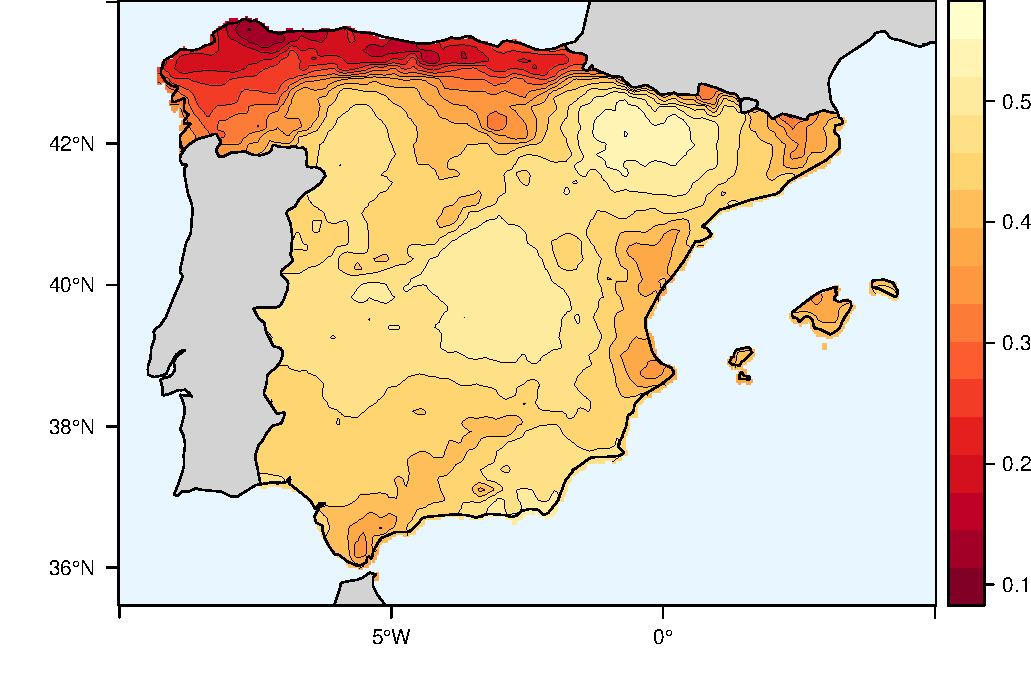
\includegraphics[height=0.3\textheight]{../figs/TwoFixed}
    }
    \par\end{centering}

  \begin{centering}
    \subfloat[Eje horizontal NS y Estático.]{%
      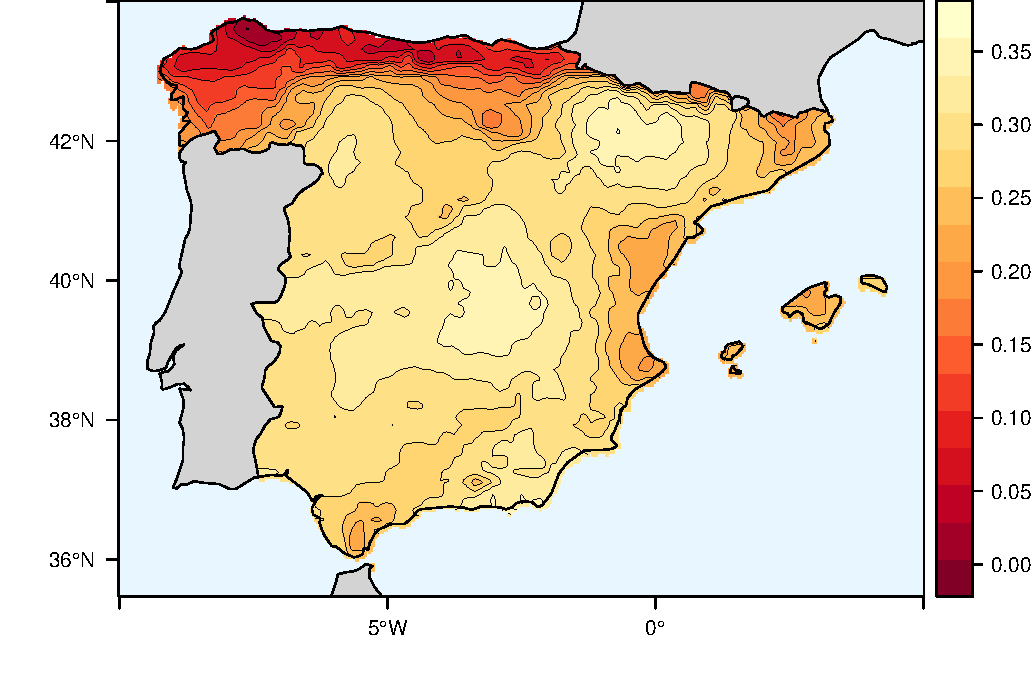
\includegraphics[height=0.3\textheight]{../figs/HorizFixed}
    }
    \par\end{centering}
  
  \begin{centering}
    \subfloat[Doble eje y Eje horizontal NS.]{%
      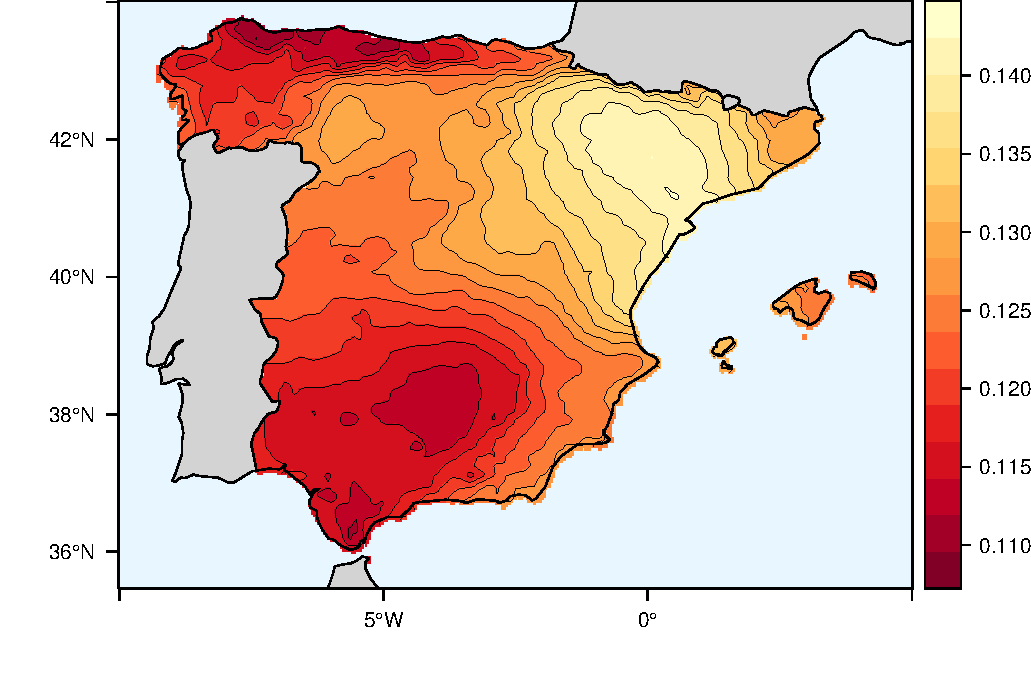
\includegraphics[height=0.3\textheight]{../figs/TwoHoriz}
    }
    \par\end{centering}
  
  \caption[Comparativa entre radiación efectiva]{Incremento de
    radiación efectiva anual por sistemas estáticos y de
    seguimiento.}
  \label{fig:ComparativaRadiación}
\end{figure}

\begin{figure}
  \begin{centering}
    \subfloat[Histograma]{%
      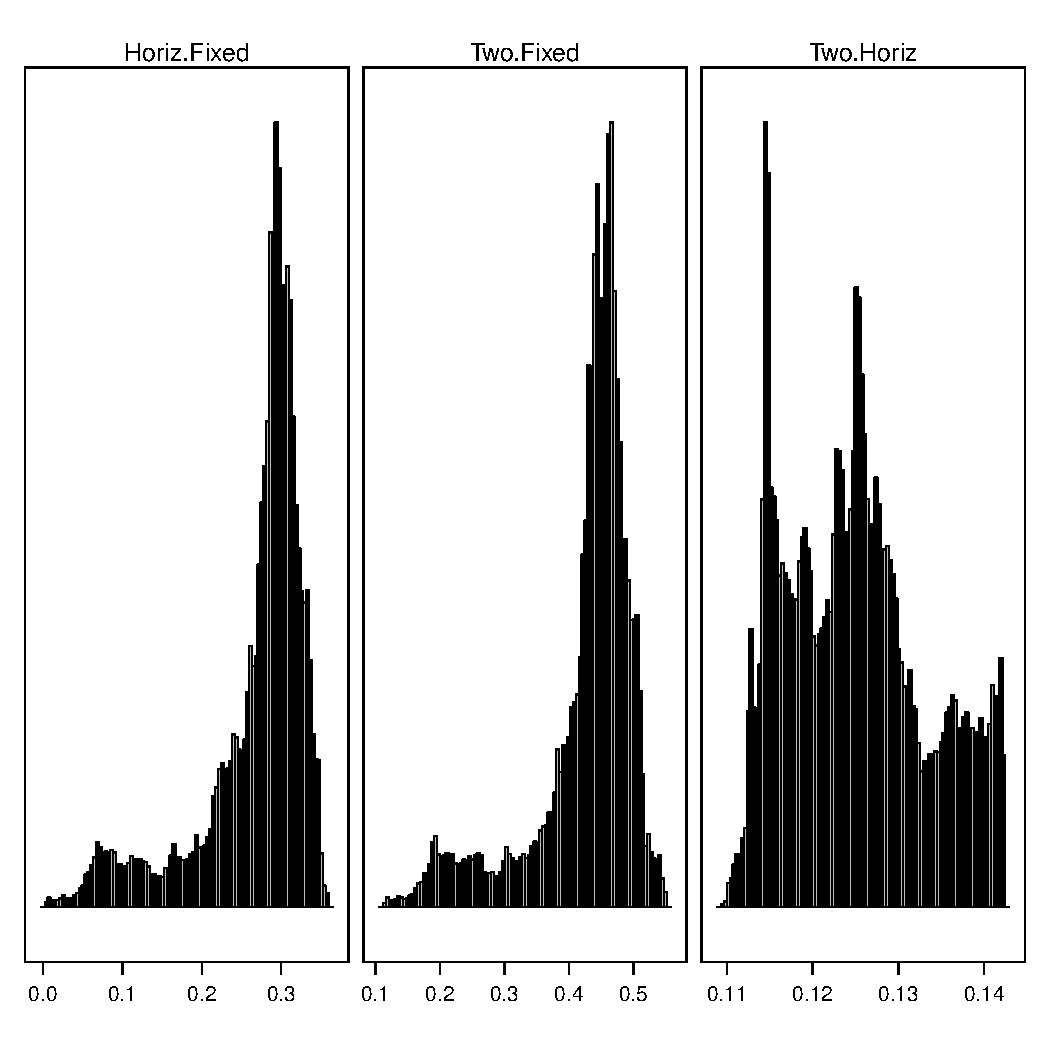
\includegraphics[height=0.45\textheight]{../figs/compSystems}
    }
    \par\end{centering}

  \begin{centering}
    \subfloat[Relación con radiación]{%
      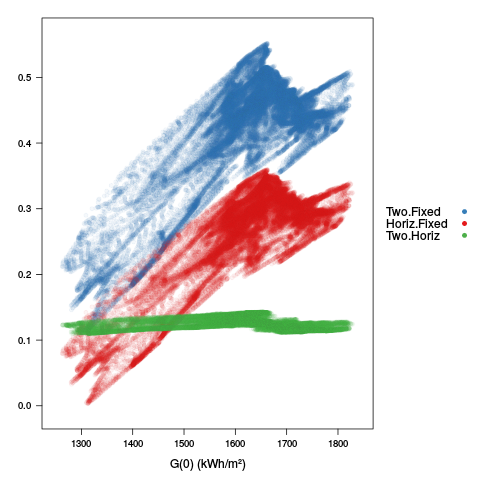
\includegraphics[height=0.45\textheight]{../figs/compSystemsG0}
    }
    \par\end{centering}
    
  \caption[Relación con radiación]{Histograma del incremento de radiación efectiva
    anual con el seguimiento, y relación con la radiación global en el plano horizontal.}
  \label{fig:HistComparativaRadiación}
\end{figure}



%%% Local Variables:
%%% mode: LaTex
%%% TeX-master: "ESF.tex"
%%% End: 